\chapter{Project Quality Management}

To ensure that the Recreation and Wellness Intranet Project meets stakeholder expectations, including those of the project sponsor, senior managers, and users, we established quality standards or requirements. These requirements align with the project's goals of increasing system usage, improving employee health, and reducing healthcare costs. Here is a list of quality standards or requirements along with brief descriptions:

\section{Quality Standards}

\begin{itemize}
    \item \textbf{User Adoption Rate}: Within the first month post-launch, we aim for a 90\% participation rate among full-time employees accessing the system. This metric serves as a barometer for gauging initial user engagement and system uptake.
    \item \textbf{Interactive Program Engagement}: We encourage active participation by ensuring that 80\% of registered employees interact with at least two wellness programs within the first six weeks. This standard underscores the importance of meaningful engagement beyond mere registration.
    \item \textbf{Health Tracking Integration}: We integrate a robust health tracking feature with at least 50\% of users syncing wearable devices or manually inputting health data within the first three months. This requirement supports the project's emphasis on empowering employees to take ownership of their health journey.
    \item \textbf{Gamified Incentive Structure}: We implement a gamified incentive system where employees can earn rewards based on achieving health milestones or participating in challenges. The clarity and attractiveness of this incentive structure should drive 60\% of employees to actively pursue rewards within the first two months.
    \item \textbf{Real-time Analytics Dashboard}: We develop a dynamic analytics dashboard providing real-time insights into participation rates, program effectiveness, and user feedback. This tool should be accessible to project stakeholders and updated weekly to inform decision-making.
    \item \textbf{Intuitive Mobile Accessibility}: We ensure seamless access and functionality across multiple devices with an emphasis on mobile usability. The system should prioritize responsive design principles to accommodate the diverse needs and preferences of users.
    \item \textbf{Data Privacy Compliance}: We adhere strictly to data privacy regulations with zero incidents of unauthorized access or breaches of employee health information. This standard underscores our organization's commitment to safeguarding sensitive data and maintaining trust.
    \item \textbf{Scalable Infrastructure}: We design the system architecture to accommodate future growth and scalability demands, with provisions for increasing user capacity and enhancing performance as needed.
    \item \textbf{Cost-Effectiveness Benchmark}: We establish a clear cost-benefit analysis framework to evaluate the project's impact on healthcare expenditure reduction. We aim for a demonstrable reduction in healthcare costs by at least 15\% within the first year of implementation.
    \item \textbf{Dynamic Feedback Loop}: We implement an agile feedback mechanism allowing users to submit suggestions, report issues, and provide ongoing input for system improvement. We regularly review and incorporate user feedback to drive iterative enhancements and optimize user experience.
\end{itemize}

\section{Quality Metrics}

Once the quality standards or requirements are established, we define metrics for measuring progress toward meeting these requirements. Here's how we measure progress on meeting the requirements:

\begin{itemize}
    \item \textbf{User Engagement}: We utilize backend analytics to track login activity and assess the frequency of employee logins within the first month post-rollout.
    \item \textbf{Adoption Rate}: We monitor the rate of adoption by tracking the number of active users engaging with the system's features within the initial six weeks.
    \item \textbf{Program Engagement}: We measure the level of engagement by analyzing the frequency and depth of interaction with various program modules within the system.
    \item \textbf{Incentive Effectiveness}: We implement regular surveys to gauge user perception of incentives and their impact on participation and motivation.
    \item \textbf{Comprehensive Reporting}: We utilize automated reporting tools to generate detailed insights into user behavior, program utilization, and outcomes.
    \item \textbf{Interface Optimization}: We conduct iterative usability tests and gather feedback to refine and enhance the system's interface for improved user experience.
    \item \textbf{Security Measures}: We perform regular security assessments and vulnerability scans to ensure robust protection against potential threats and breaches.
    \item \textbf{Performance Monitoring}: We utilize performance monitoring tools to track system responsiveness, uptime, and overall performance metrics.
    \item \textbf{Health Outcomes Evaluation}: We evaluate the system's impact on health outcomes by analyzing relevant health indicators and comparing pre- and post-implementation data.
    \item \textbf{Feedback Analysis}: We analyze feedback data to identify trends, address user concerns, and continuously improve the system's functionality and user experience.
    \item \textbf{Program Effectiveness}: We assess the effectiveness of various health programs by tracking key metrics such as participation rates, behavior change, and health improvements over time.
\end{itemize}

\section{Pareto chart}

\begin{tabular}{|l|r|r|}
\hline
\textbf{Requested Programs} & \textbf{Number of Requests} & \textbf{\% of Requests} \\
\hline
Walking program & 7115 & 24\% \\
Volleyball program & 2054 & 7\% \\
Weight reduction class & 8875 & 30\% \\
Stop smoking class & 4889 & 17\% \\
Stress reduction class & 1894 & 6\% \\
Soccer program & 3297 & 11\% \\
Table tennis program & 120 & 0\% \\
Softball program & 976 & 3\% \\
\hline
\textbf{Total} & \textbf{29220} & \textbf{100\%} \\
\hline
\end{tabular}

\begin{figure}[h!]
    \centering
    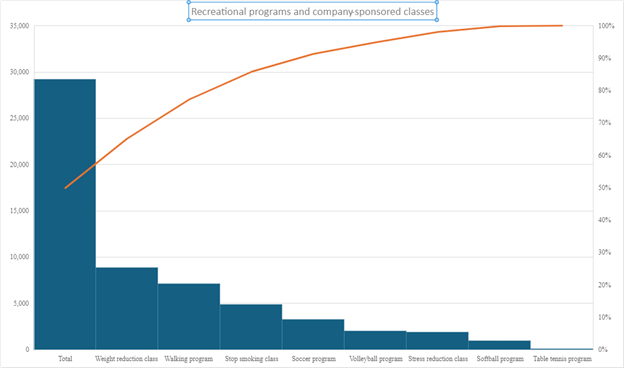
\includegraphics[width=\textwidth]{images/image.png}
    \caption{Program Requests Distribution}
\end{figure}